% 2009 年辽宁卷理科第 22 题【A】：△ABC 的外接圆，D 是劣弧 AC 上的点，延长 BD 至 E。
% 来源 PDF：普通高考/2009/2009辽宁理.pdf，SHA256 5ae9708acfe7def5bddd60a34d1474cfa2e2c20a39d130255e0e4393093accad
% 原页：第 2 页（A3 三栏）第 3 栏上部，印刷页 538。
% 重绘依据：A 在圆上最高处，B、C 在下方左右对称（AB=AC），D 在 A 与 C 之间的劣弧上，
%   B、D、E 共线且 E 在 D 的延长线上；连 AB、AC、AD、BC、CD，并延长 BD 至 E。
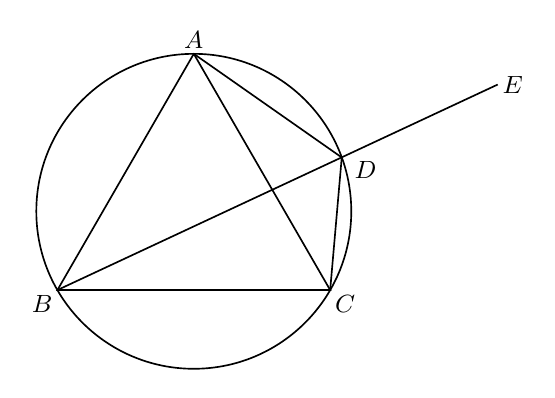
\begin{tikzpicture}[scale=1.0, semithick, every node/.style={inner sep=1.5pt, font=\small}]
  \coordinate (O) at (0,0);
  \coordinate (A) at (0,2);
  \coordinate (B) at (-1.732,-1);
  \coordinate (C) at (1.732,-1);
  \coordinate (D) at (1.879,0.684);
  \coordinate (E) at (3.86,1.61);
  % 外接圆
  \draw (O) circle (2);
  % 三角形与相关线段
  \draw (A) -- (B) -- (C) -- (A);
  \draw (A) -- (D);
  \draw (C) -- (D);
  \draw (B) -- (E);
  % 顶点标注
  \node[above] at (A) {$A$};
  \node[below left] at (B) {$B$};
  \node[below right] at (C) {$C$};
  \node[right] at (1.98,0.52) {$D$};
  \node[right] at (E) {$E$};
\end{tikzpicture}
